\documentclass[11pt,twocolumn]{article}
\usepackage{amsmath}
\usepackage[margin=1in]{geometry}
\usepackage{graphicx}
\usepackage{import}
\usepackage{subfig}

\title{Vision-Based Autonomous Ground Vehicle Navigation}
\date{March 31, 2011}
\author{
	Michael Koval \\
	mkoval@eden.rutgers.edu \\
	Electrical and Computer Engineering
}

\begin{document}
\maketitle

\section{Introduction}
\label{sec:intro}
% 1. Overall description of IGVC
The Intelligent Ground Vehicle Competition (IGVC) is an international
collegiate robotics competition that tasks teams of undergraduate students to
design, build, and program a fully autonomous mobile ground vehicle.
Specifically, a successful entry must be capable of navigating through a narrow
obstacle course, travelling between  global positioning system (GPS) scattered
throughout a field, and responding to Joint Architecture for Unmanned Systems
(JAUS) messages ~\cite{igvc11}.

% 2. Importance of Perception
In each of these tasks, the robot is provided witih only the destination
waypoint and has no a priori no knowledge of the course's topology. Safely
reaching the goal without crossing a course boundary or hitting an obstacle
requires that the robot both build a map of its environment and use the map to
plan through drivable regions to the destination. This is further complicated
by the use of only narrow, white painted lines to delimit the course boundaries
and the addition of a large variety of road obstacles to obstruct the path,
including cones, barriers, potholes, and switchbacks
~\cite{igvc11}.

% 3. Overview
Finding these obstacles has historically been accomplished using a combination
of a scanning laser range finder (LIDAR) and computer vision to build a local
map of nearby obstacles and lines ~\cite{princeton08} ~\cite{delaware08}.
Before discussing specific algorithms for computing this information, Section
~\ref{sec:robot} provides a brief introduction to the hardware and software in
use on the Rutgers Navigator: Rutgers University's 2011 IGVC entry. The
remainder of this is split into two major sections: the use of stereo vision
for obstacle detection (Section ~\ref{sec:stereo}) and the monocular image
processing used to to track the course boundary lines (Section
~\ref{sec:line}). Finally, Section ~\ref{sec:future} addresses planned
improvements to the vision system and Section ~\ref{sec:econ} discusses how
robotics can assist in the recovery from major environmental disasters, such as
the recent earthquake off the cost of Japan.

\section{Rutgers Navigator}
\label{sec:robot}
% 1. Brief discussion of mechanical design
Designed specifically for rugged outdoor use and modularity, the Rutgers
Navigator is constructed entirely out of 80/20 extrusion and custom-machined
alumninum stock. This provides a strong, light\footnote{Approximately 100 lb
empty and 150 lb fully loaded.} frame that is much easier to modify than the
equivalent welded steel frame. This chassis is supported by three wheels: two
powered front wheels that are mounted on a wish bone suspension for improved
stability and free-spinning rear castor chosen specifically to reduce friction
while turning.

\begin{figure}
	\center
	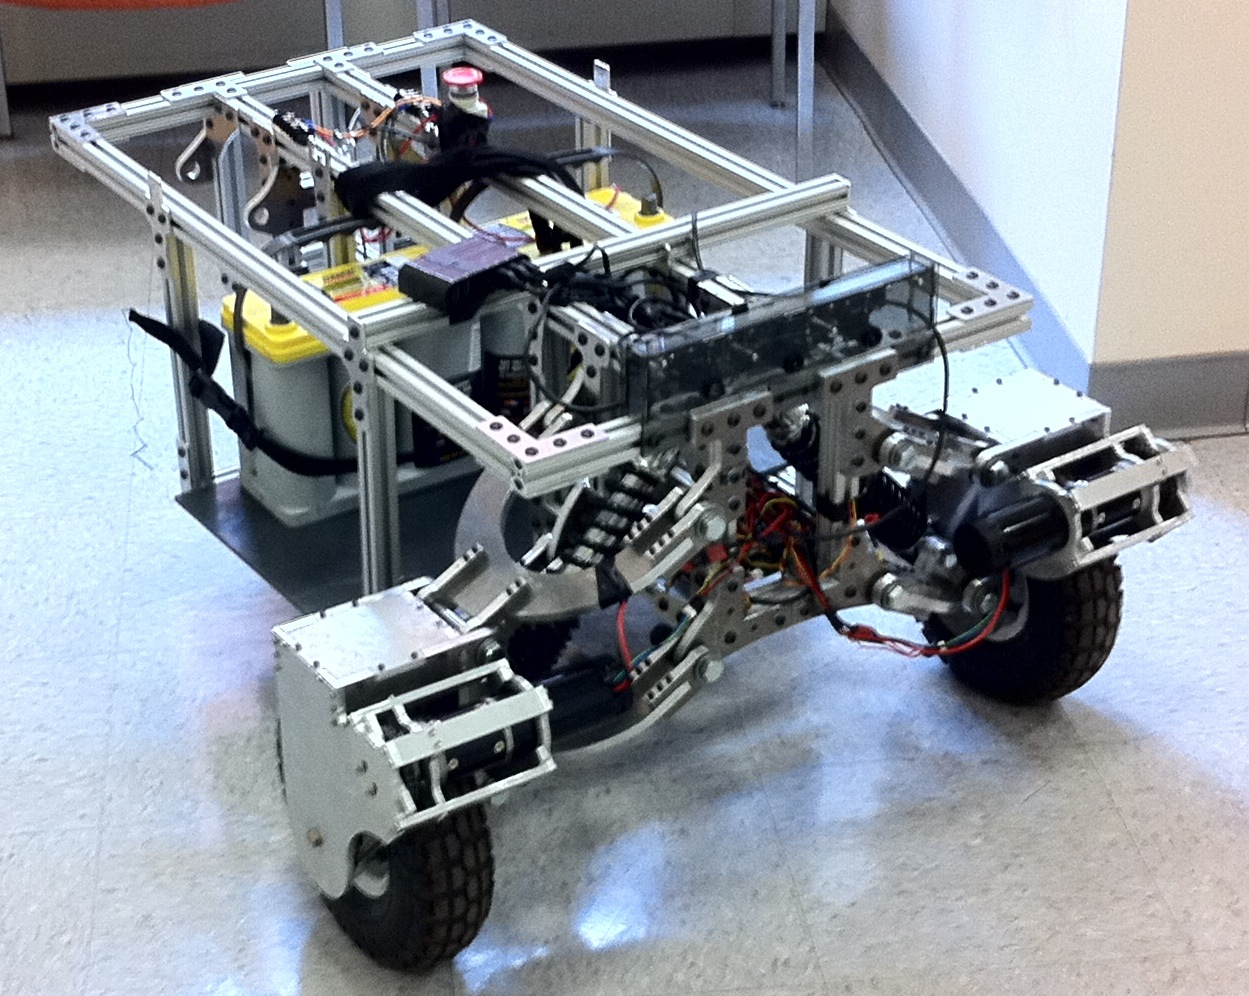
\includegraphics[width=\linewidth]{include/robot-photo}
	\caption{Rutgers Navigator robot}
	\label{fig:robot-photo}
\end{figure}

% 2. Sensing capabilities
\subsection{Sensing Capabilities}
\label{sec:robot-sensors}
Each of the drive motors that attached to the drive wheels are equipped with
internal hall-effect quadrature encoders to measure wheel speed and a current
sensor to monitor power consumption. The local odometry information captured by
the wheel encoders is combined with the data produced by a nine-axis intertial
measurement unit (IMU) that includes an accelerometer, gyroscope, and magnetic
compass to estimate the robot's motion. Conversely, the robot's absolute
position is found using a high-end Novatel differential global positioning
system (DGPS) that is accurate within 50 cm under normal operation and 10 cm
when using OmniStar's correction service ~\cite{omnistar}.

As was discussed in Section ~\ref{sec:intro}, precise knowledge of the robot's
position is not sufficient to successfully complete the challenges. Obstacles
in the robot's environment are detected using a Hokuyo LIDAR and the custom
trinoculur stereo vision system that is discussed in detail in Section
~\ref{sec:stereo}. Combining the planar point cloud captured by the LIDAR with
the full three-dimensional information produced by stereo camera results in an
aggregate point cloud with both the field of view and granularity necessary to
successfully avoid obstacles.

\subsection{Software Architecture}
\label{sec:robot-software}
Interaction between the robot's individual software components is implemented
using the Robot Operating System (ROS), a framework developed by Willow Garage
to promote code reuse in robotics. Besides providing a common interface to
libraries such as OpenCV and PointCloud Library (PCL), ROS encourages the
separation of software into a graph of loosely-coupled \textit{nodes} that
communicate over TCP/IP sockets ~\cite{ros}. Because each node
\textit{subscribes} to its inputs and \textit{publishes} its outputs with no
global knowledge of the system, it is possible to reuse nodes without ever
modifying their internals.

\begin{figure}
	\centering
	\includegraphics[width=\linewidth]{include/robot-software-vision}
	\caption{Computer vision software subsystem.}
	\label{fig:robot-vision}
\end{figure}

Using the concept of a node to model the flow of data through the computer
vision subsystem produces the graph shown in Figure ~\ref{fig:robot-vision}.
Within this graph, there are three distinct processing piplines: stereo vision,
monocular lane tracking, and monocular object recognition. As its name
suggests, the \textit{stereo vision} pipeline (Section ~\ref{sec:stereo} uses
triplets of synchronized images to generate a three-dimensional point cloud
later used to identify obstacles. The monocular \textit{line tracking} (Section
~\ref{sec:line}) pipeline identifies white boundary lines in each input image
and tracks their positions relative to the robot over time. Finally, the
\textit{object recognition} pipeline identifies purely visual targets and
obstacles such as ``simulated potholes''\footnote{Ellipses placed on the grass
to simulate real potholes.} and target flags.

\section{Stereo Vision}
\label{sec:stereo}
%
%
%
% TODO: Comparison with Hokoyu
%
%
%

\subsection{Synchronization}
\label{sec:stereo-sync}
Stereo vision on a mobile robot is a non-trivial problem that has traditionally
required custom machine vision hardware with two or more hardware-synchronized
cameras. Because standard stereo reconstruction assumes that the images from
each camera are captured of a fixed scene from multiple viewpoints, any motion
that occurs between the cameras capturing frames is interpreted as an
unexpected change in the system's baseline. This change in baseline invalidates
the system's extrinsic calibration\footnote{Capturing images at 30 Hz while
moving at 10 mph could change the baseline by up to 7 cm.}, causing the quality
of the rectification to decrease and the distances to be distorted by the
robot's velocity ~\cite{unsync}.

\begin{figure*}
	\centering
	\subfloat[Unsynchronized \texttt{VSYNC}]{
		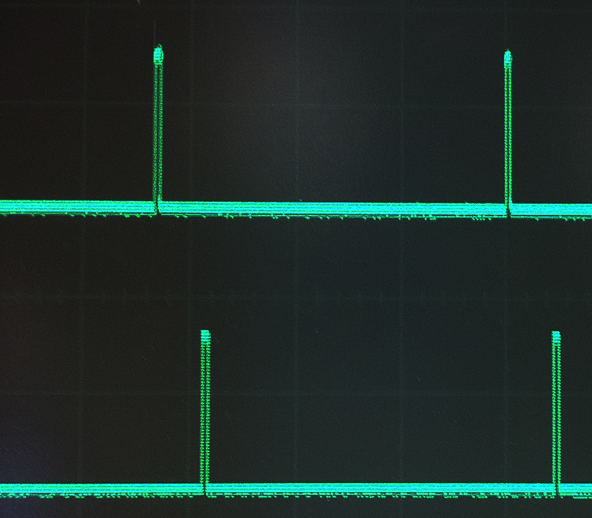
\includegraphics[width=0.24\textwidth]{include/unsync-scope}
		\label{fig:stereo-sync-hard1}
	}
	\subfloat[Synchronized \texttt{VSYNC}]{
		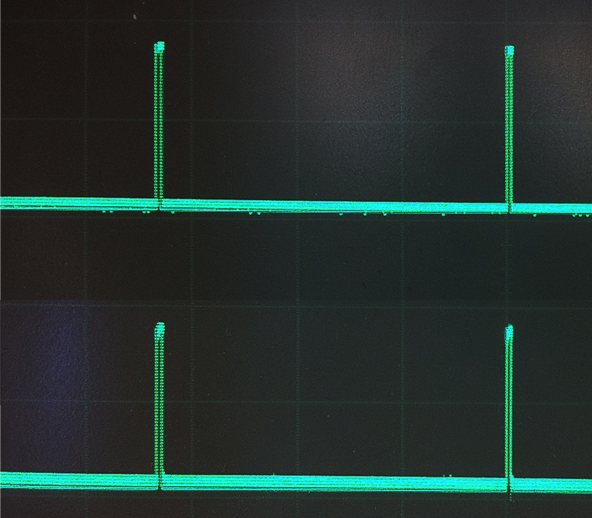
\includegraphics[width=0.24\textwidth]{include/sync-scope}
		\label{fig:stereo-sync-hard2}
	}
	\subfloat[Unsynchronized Frames]{
		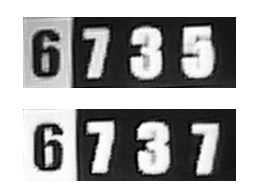
\includegraphics[width=0.24\textwidth]{include/unsync-img}
		\label{fig:stereo-sync-soft1}
	}
	\subfloat[Synchronized Frames]{
		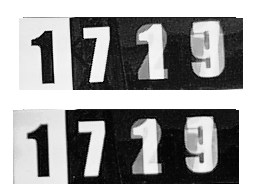
\includegraphics[width=0.24\textwidth]{include/sync-img}
		\label{fig:stereo-sync-soft2}
	}
	\caption{
		Verification of hardware and software camera synchronization for two
		Playstation Eye cameras. Note how only the synchronized cameras share a
		common \texttt{VSYNC} clock and capture identical readings of a
		millisecond resolution timer.
	}
	\label{fig:stereo-sync}
\end{figure*}

Hardware synchronization has been traditionally limited to specialized cameras,
such as the Bumblebee series of stereo cameras. Thankfully, the inexpensive
Playstation Eye camera is built on the high-end OmniVision OV7720 chipset,
which can be hardware-synchronized using the exposed frame clock input
(\texttt{FSIN}) and output (\texttt{VSYNC}) pins ~\cite{omnivision}. By
shorting one camera's (the \textit{master}) \texttt{VSYNC} pin to the other
cameras' (the \textit{slaves}) \texttt{FSIN} pins, the cameras are forced to
share a common clock. To reduce the risk of a large potential difference from
damaging the cameras, each camera was also modified to share a common ground.

This hardware synchronization guarantees that the cameras capture images
simultaneously, but does not guarantee that the frames will remain synchronized
after the USB transfers to the computer. Making direct use of the Video4Linux
kernel module, synchronization was achived by fuzzy-matching of the the USB
transfer timestamps\footnote{\texttt{https://github.com/mkoval/stereo\_webcam}}
assigned to the memory-mapped I/O by the kernel driver.

Hardware synchronization was verified by probing each camera's \texttt{VSYNC}
pin with an osilloscope (Figures ~\ref{fig:stereo-sync-hard1} and
~\ref{fig:stereo-sync-hard2}) and confirming that all three clocks were in
phase. The software synchronizaton was additionally verified by simultaneously
capturing images of a millisecond resolution timer (Figures
~\ref{fig:stereo-sync-soft1} and ~\ref{fig:stereo-sync-soft2}. Mounted in a
custom polycarbonate case, three of these hardware-synchronized Playstation Eye
cameras serve as the backbone of the Navigator's trinocular vision system.

\subsection{Baseline Selection}
\label{sec:stereo-mux}
Selecting the optimal baseline for a stereo system is a balance of two
opposing, but equally important, factors: field of view and precision.
Decreasing the baseline increases the shared field of view of the two cameras
at the cost of less precise distance measurements. Conversely, increasing the
baseline trades a decrease in field of view for better precision at each
range. Using a trinocular system allows the software to select between
two different baseilnes: a \textit{narrow} baseline that uses the left and
center cameras and a \textit{wide} baseline that uses the left and right
cameras. Using the trinocular Bumblebee3 Stereoscopic Camera as a model, the
\textit{narrow stereo} baseline was set to 10 cm and the \textit{wide stereo}
baseline was set to 20 cm.

\begin{figure*}
	\centering
	\subfloat[Multiplexed Point Cloud]{
		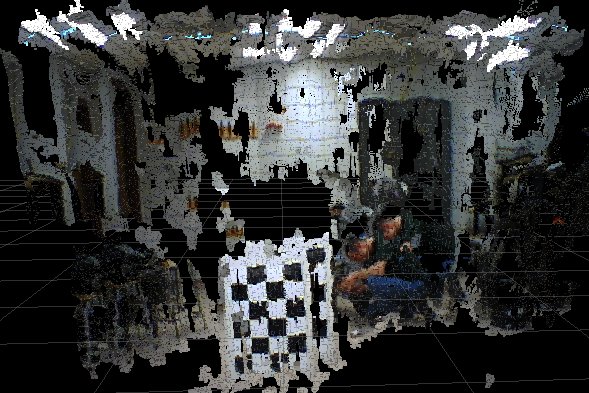
\includegraphics[width=0.5\linewidth]{include/stereo-both}
	}
	\subfloat[Reconstruction Error]{
		\subimport{include/}{stereo-dist}
	}
	\caption{
		Reconstructed point cloud using stereo multiplexing. Differences in the
		camera's rectification and reconstruction accuracy cause a small
		rotation in the reconstructed point cloud.
	}
	\label{fig:stereo-dist}
\end{figure*}

\subsection{Reconstruction Algorithm}
\label{sec:stereo-algo}
Due to the use of ROS as the basis for the Navigator's software architecture
(Section ~\ref{sec:robot}), the actual stereo reconstruction is done using the
standard \texttt{stereo\_image\_proc} ROS node. Before being processed for
point correspondances, the pair of input images is rectified, regions of low
texture are masked out, and a Sobel filter is applied to amplify texture
~\cite{stereo}. Each pixel in the left image is matched to the most similar
pixel in the corresponding row in the right image using a sum-of-squared
difference (SSD) block-matching algorithm ~\cite{stereo}, producing that
pixel's disparity. This disparity is then converted to a three-dimensiona point
using the camera's intrinsic parameters.

While more efficient than the graph-cut based alternatives, ~\cite{stereo} the
SSD block-matching algorithm implemented in the ROS
\texttt{stereo\_image\_proc} is still extremely computationally intensive.
Considering that the narrow and wide baselines have a great deal of overlap,
much of this computation is wasted: many of the three-dimensional points will
be duplicates. Quickly alternating between the two baselines, or
\textit{baseline multiplexing}, reduces the computational load of the
trinocular stereo system to nearly the same as the binocular equivalent. In
practice, baseline multiplexing allows the entire vision system to process
images at approximately 10 Hz.

\subsection{Error Analysis}
\label{sec:stereo-error}
After calibrated with the ROS \texttt{camera\_calibration} package, the
accuracy of both baselines was evaluated by comparing the actual depth of a
calibration chessboard to the reconstructed distances. Plotting the
reconstructed distance against the actual distance at distances from 0 to 8
meters (Figure ~\ref{fig:stereo-dist}) confirms this analysis. At short
distances, the narrow stereo's dead zone of 0.9 m is substantially less than
the wide stereo's dead zone of 1.6 m. As distance increases beyond 3 meters,
however, the narrow stereo becomes much less accurate and the wide stereo is
superior.

\section{Lane Tracking}
\label{sec:line}
For both the navigation and GPS challenges, the drivable region of the course
is delimited by a three inch wide line painted on the grass or asphalt.
Robustly identifying and tracking these lane boundary lines is an extremely
difficult problem that has been the primary cause of disqualifications in
previous years of competitions. For example, 28 out of 29 competitors were
disqualified failing to move, leaving the course, or striking an obstacle
before five minutes time limit elapsed in the 2010 IGVC.
~\cite{igvc_results10}.

The algorithm discussed below is a modified version of the algorithm used by
Massachusettes Institute of Technology's entry into the DARPA Grand Challenge.
In this algorithm, a color image of the course undergoes a color spae
transformation to emphasize white regions of the image (Section
~\ref{sec:line-color}). The grayscale output of the color space transformation
is then filtered using a matched pulse-width filter (Section
~\ref{sec:line-filter}) and compressed with non-maximal supression (Section
~\ref{sec:line-max}). These local maxima are then transformed into the world
coordinate frame and are directly used for navigation ~\cite{huang_thesis}
~\cite{huang_paper}.

\begin{figure*}[t]
	\centering
	\subfloat[Original Image]{
		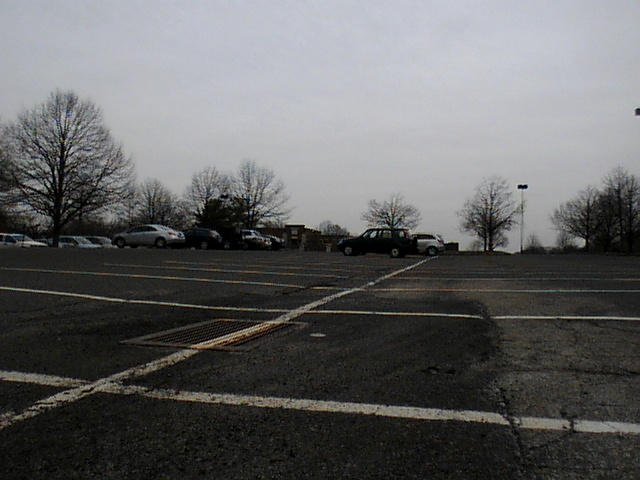
\includegraphics[width=0.45\linewidth]{include/line-orig}
	}
	\subfloat[Color Space Transformation]{
		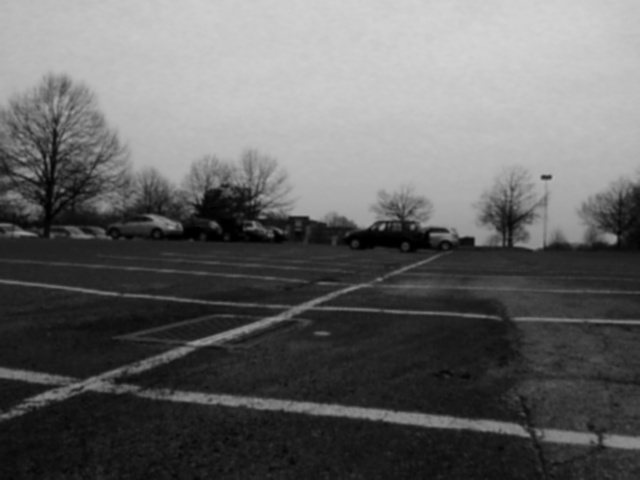
\includegraphics[width=0.45\linewidth]{include/line-pre}
	}
	\\
	\subfloat[Matched Pulse-Width Filter]{
		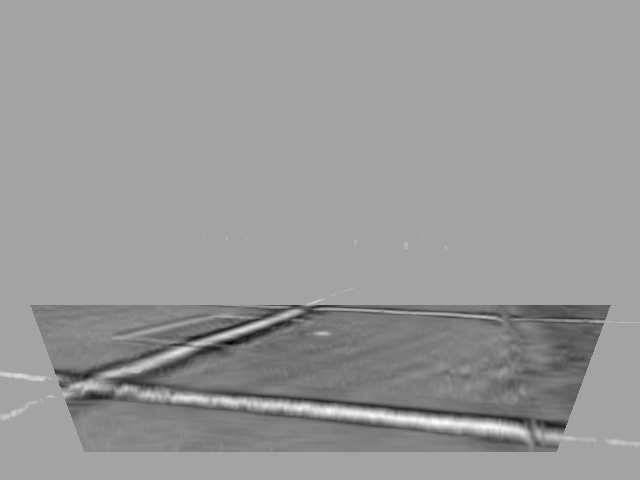
\includegraphics[width=0.45\linewidth]{include/line-filter}
	}
	\subfloat[Non-Maximal Suppression]{
		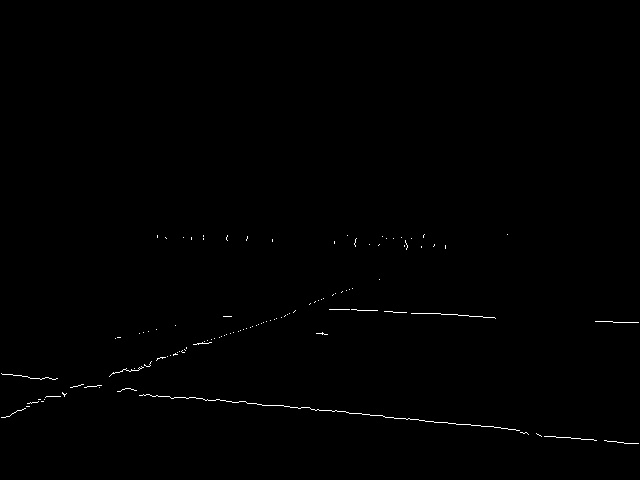
\includegraphics[width=0.45\linewidth]{include/line-max}
	}
	\caption{Intermediate stages of the line detection algorithm.}
	\label{fig:line-all}
\end{figure*}

\subsection{Color Space Transformation}
\label{sec:line-color}
Using \textit{a priori} knowledge that the lines are white, the first step
towards effectively isolating them from their surroundings is to convert the
rectified color image into a monochromatic color space where white is
amplified. Because white is inheriently of high intensity and low saturation,
the hue-saturation-value (HSV) color space is a natural choice. If the original
image, $I_{orig}$, has the 8-bit HSV channels $H(x,y)$, $S(x, y)$, and $V(x,
y)$, define the pre-processed image $I_{pre}$ to be
\begin{equation*}
	I_{pre}(x, y) = \min\left\{255 - S(x, y), V(x, y)\right\}
\end{equation*}
for each pixel $(x, y)$ in $I_{orig}$.

\subsection{Matched Pulse-Width Filter}
\label{sec:line-filter}
Because the lines on the course are known to be uniformly three inches wide, an
obvious approach for isolating them from other objects is to use a digital
\textit{pulse-width filter} that is of the same width. Unfortunately, the
effects of perspective projection mean that the apparent width of lines in the
image depend upon their distance from the camera. To obtain useful output, such
a filter must be properly \textit{matched} to expected width of the line at
each point in the image ~\cite{huang_thesis} ~\cite{huang_paper}.

Calculating this width requires knowledge of the three-dimensional point
corresponding to each pixel in the image. Assuming that the ground plane is
known and is parameterized by point $P$ and normal $n$, the three-dimensional
point $P$ that corresponds to pixel $p$ satisifes both
\begin{align*}
	(P - P_0) \cdot n          &= 0 \\
	\lambda M^{-1}_{int} p - P &= 0,
\end{align*}
where $M_{int}$ is the camera's intrinsic matrix and $\lambda$ is an arbitrary
constant.

Solving for $\lambda$ results in a closed-form expression containing
only known parameters. Substituting this value into the equation of the
line yields an intersection point of
\begin{equation*}
 	P = \left(\frac{n \cdot P_0}{n \cdot M^{-1}_{int} p}\right) M^{-1}_{int} p.
	\label{eqn:line-point}
\end{equation*}
Using the new-found knowledge of point $P$, the length of an arbitrary real-world
vector projected into the image at point $p$ is
\begin{equation}
	\delta = ||M_{int} P - M_{int} (P + \Delta)||_2
	\label{eqn:line-width}
\end{equation}
where $\delta$ is the image distance corresponding to a change in world
coordinates by the vector $\Delta$ and $||\cdot||_2$ denotes the Euclidean
norm. Note that this is not equivalent to $||M_{int}\Delta||_2$ because of the
division implicit in the use of homogeneous coordinates.

\begin{figure}
	\centering
	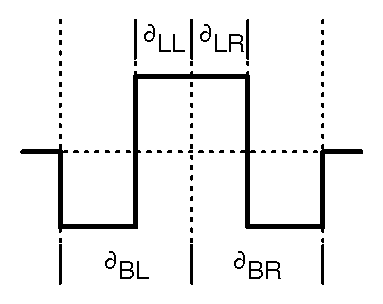
\includegraphics[width=0.6\linewidth]{include/line-sketch}
	\caption{Sketch of the matched pulse-width filter's kernel.}
	\label{fig:line-sketch}
\end{figure}

Using this equation, the four distances of interest depicted in Figure
~\ref{fig:line-sketch} are projected into the image using Equation
~\ref{eqn:line-width}. Of these four distances, $\delta_{LL}$ and $\delta_{LR}$
correspond to the left and right edges of the line, respectively. Similarly,
$\delta_{BL}$ and $\delta_{BR}$ correspond to the expected total width of the
filter (including a dead zone around the line). Note that the filter is only
symmetric (i.e. $\delta_{LL} = \delta{LR}$ and $\delta_{BL} = \delta_{BR}$) for
the horizontal filter kernel. The vertical filter is assymetric and shifted due
to the effect of perspective projection.

Once the four widths have been projected into the image, a filter kernel is
constructed such that each of the negative \textit{supports} sums to $-0.5$
and the central \textit{pulse} sums to $+1.0$. This causes the filter to have
a zero response on solid color and to only respond strongly to lines of the
correct width and orientation. The region surrounding each pixel in the image
is convolved with both the horizontal and vertical matched filters and the
responses are ready for post-processing.

\subsection{Non-Maximal Suppresion}
\label{sec:line-max}
The matched pulse-width filter is extremely effective at isolating the line in
the image, but does not produce a clean enough output to be directly used for
model-fitting. In particular, the nature of digital filters guarantees that
there will be weak, spurious responses near true positives.

Inspired by Canny edge detection, non-maximal supression is an effective and
computationally efficient way of reducing such a response to a single point.
Considering the rows of the horizontally filtered image and the columns of the
vertically filtered image, a pixel is considered a maximum if and only if it
has a higher filter response than both of its neighbors. The maxima are then
thresholded to discard those that do not exhibit a sufficiently strong filter
response. This threshold was tuned to favor false positives and was set to
approximately 15\% of the filter's maximum response.

\subsection{Error Analysis}
\label{sec:line-error}
This algorithm is largely rooted in physical constants, it is relatively sensitive to the ground plane having an incorrect orientation. Constructing the matched pulse-width filters succeeds even with large variations in the ground plane, but those filters no longer match the width of the line in the image. Even worse, the detected line points in the world appear at the wrong distance from the image. Tested on both simulated data and real data, the algorithm appears very effective at identifying lines even in noisy environments (e.g. the parking lot in Figure ~\ref{fig:line-all}).

\section{Conclusion}
\label{sec:conclusion}
After extensive testing of the custom stereo camera using an oscilloscope, a millisecond resolution timer, and outdoor data, it is clear that the three cameras are well synchronized. This synchronization translates into an extremely high quality reconstruction while the robot is moving, giving it the rich three-dimensional information required for path planning. Applying a matched pulse-width filter to detect the lines bordering the field succesfully corrects for the effects of perspective transform and reliably detects both horizontal and vertical lines in the image. 

\section{Future Work}
% TODO

\label{sec:future}
% 1. Obstacle detection using the stereo point cloud
% 2. Use stereo depth information to mask line false positives
% 3. Stereo and/or IMU-based ground plane detection
% 4. Use normal vectors to fit bicubic splines
% 5. Basic object recognition for flags, potholes, and road obstacles
% 6. Ground plane detection with stereo/kinect/imu

\section{Current Trends in Robotics}
\label{sec:econ}
% 1. Search and Rescue
The recent Japanese earthquake and tsunami was one of the worlds' most
devestating natural disastors. ~\cite{????} While the Japanese people's
efficient response captivated international news, it rapidly became clear
old-school search and rescue methods are much less effective on the national
and international scale. Each volunteer that climbs through the debris
generated by the earthquake and tsunami is capable of moving only a few miles
per hour and is limited to those areas that are deemed sufficiently safe to
walk.

All of the traditional problems associated with search and rescue, including
cramped quarters, unstable conditions, and the massive search area are only
problems for a human who are performing the search. Small, agile, tank-like
robots designed specifically driving over rubble feature. % TODO ...

% 2. Infastructure Evaluation and Repair
Once the search and rescue response is complete, a country struk by a natural
disaster must begin repairing its infastructure. With the amount of damage
caused in natural disaster of this magnitude, the situation quickly becomes one
of triage. The most important pieces of infastructure must be repaired first to
restore power, clean water, and electricity to the recovering nation. Improving
the utility worker's ability 


% 3. HAZMAT Situations

% 4. Challenges


\section{Acknowledgements}
This project would not have been possible without the support of Dr. Predrag
Spasojevic as our faculty advisor or the help of the members of Rutgers IEEE
Student Branch. I am particulary grateful for Adam Stambler's excellent
leadership, Peter Vasilnak's mechanical design, and the faculty support of Dr.
Kristin Dana, Joe Lippencott, Steve Orbine, John Scafidi, and Dr. Stuart
Shalat. I would also like to thank our sponors: Rutgers Engineering Governing
Council, Knotts Corporation, 80/20 Inc., Optima Batteries, Github, IEEE Region
1, Novatel, and Omnistar.

\appendix
\section{Source Code}
Digital access to all code is available online upon request via a private
Github respository.

% 1. stereo_webcam
% 2. stereo_mux
% 3. line_detection
% 4. line_tracker
% 5. camera_calibration modification (???)

\end{document}
